%
% hardware.tex
%
% Copyright (C) 2021 by SpaceLab.
%
% EPS 2.0 Documentation
%
% This work is licensed under the Creative Commons Attribution-ShareAlike 4.0
% International License. To view a copy of this license,
% visit http://creativecommons.org/licenses/by-sa/4.0/.
%

%
% \brief Hardware project chapter.
%
% \author Gabriel Mariano Marcelino <gabriel.mm8@gmail.com>
% \author Yan Castro de Azeredo <yan.ufsceel@gmail.com>
%
% \institution Universidade Federal de Santa Catarina (UFSC)
%
% \version 0.2.0
%
% \date 2021/02/16
%

\chapter{Hardware} \label{ch:hardware}

The EPS2 is a 4 layer 1.6mm thick PCB with FR-4 dieletric. The module doesn't have any impedance control requirements, for this reason the layer stackup has 1oz (0.0347mm) thickness in inner and outer copper layers. In the following sections, the hardware design, interfaces, and standards are described in detail. Section are devided by subsystem blocks, following the diagrams present on \autoref{fig:mcu-block-diagram} and \autoref{fig:power-block-diagram}. The \autoref{fig:pcb-top}, \autoref{fig:pcb-bottom} and \autoref{fig:pcb-side} presents the 3D rendered images of the top, bottom and side views of the board, respectively.

\begin{figure}[!ht]
    \begin{center}
        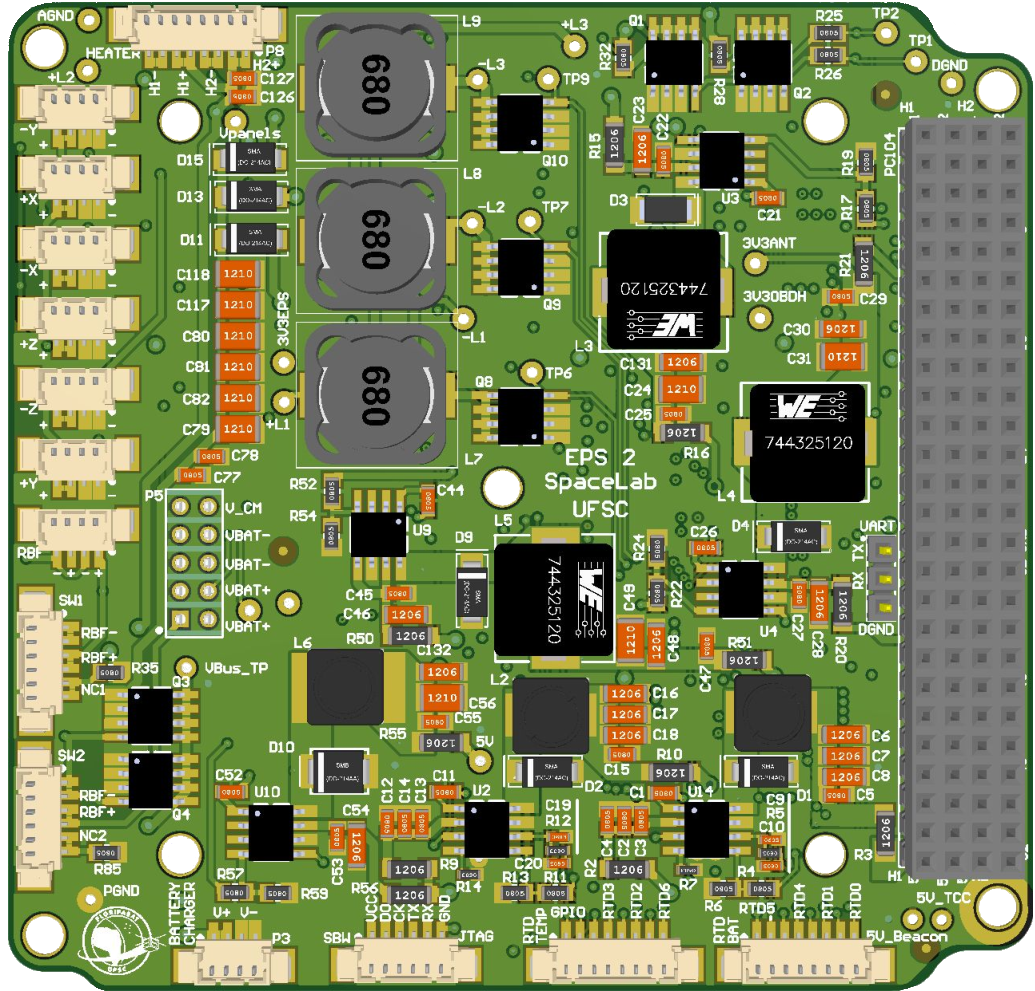
\includegraphics[width=93mm]{figures/eps2-pcb-top.png}
        \caption{Top side of the PCB.}
        \label{fig:pcb-top}
    \end{center}
\end{figure}

\begin{figure}[!ht]
    \begin{center}
        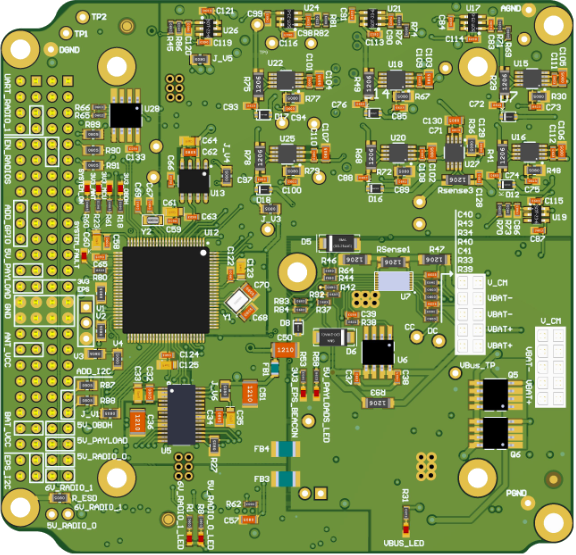
\includegraphics[width=93mm]{figures/eps2-pcb-bottom.png}
        \caption{Bottom side of the PCB.}
        \label{fig:pcb-bottom}
    \end{center}
\end{figure}

\begin{figure}[!ht]
    \begin{center}
        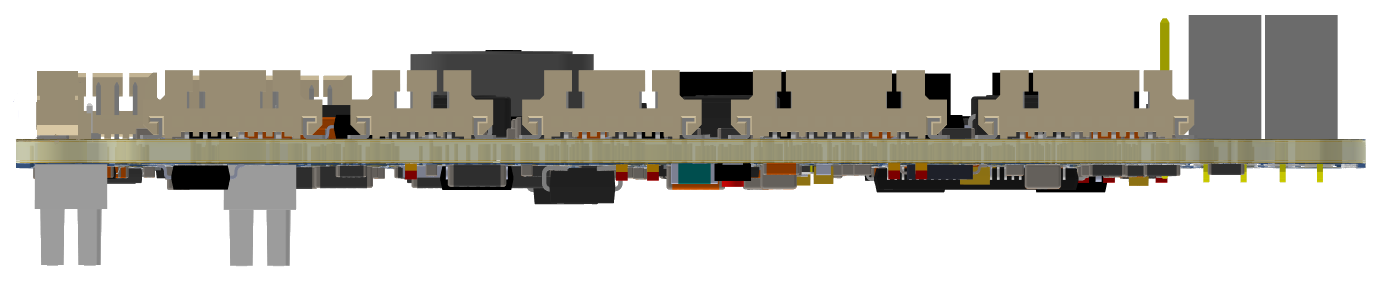
\includegraphics[width=93mm]{figures/eps2-pcb-side.png}
        \caption{Side view of the PCB.}
        \label{fig:pcb-side}
    \end{center}
\end{figure}

\section{Interfaces}

The \autoref{fig:diagram-interfaces} presents the board interfaces, which consists of communication with other modules, debug access points, and internal peripherals. From the perspective of the microcontroller, there are 5 individual communication buses and the JTAG interface (Spy-Bi-Wire), in the \autoref{tab:interfaces}: A1-SPI (dedicated for RTD analog readings with ADS1248); A0-UART (dedicated for Beacon Radio); A2-UART (dedicated for debug); B0-I2C (dedicated for DS2777); B2-I2C (dedicated for OBDH); From the External Interface (IIP) can be acquired UART log messages for debbuging via USB without the use of an external UART to USB converter. The SPI comunicaton bus it actually an dedicated internall channel for the EPS MCU (master) to the ADS1248 (slave) ADC IC, the analog readings from BAT4C module (a.k.a Battery DaughterBoard) were also represented to show where the RTDs readings come from. \autoref{tab:usci-config} shows the interfaces configuration.

\begin{figure}[!ht]
    \begin{center}
        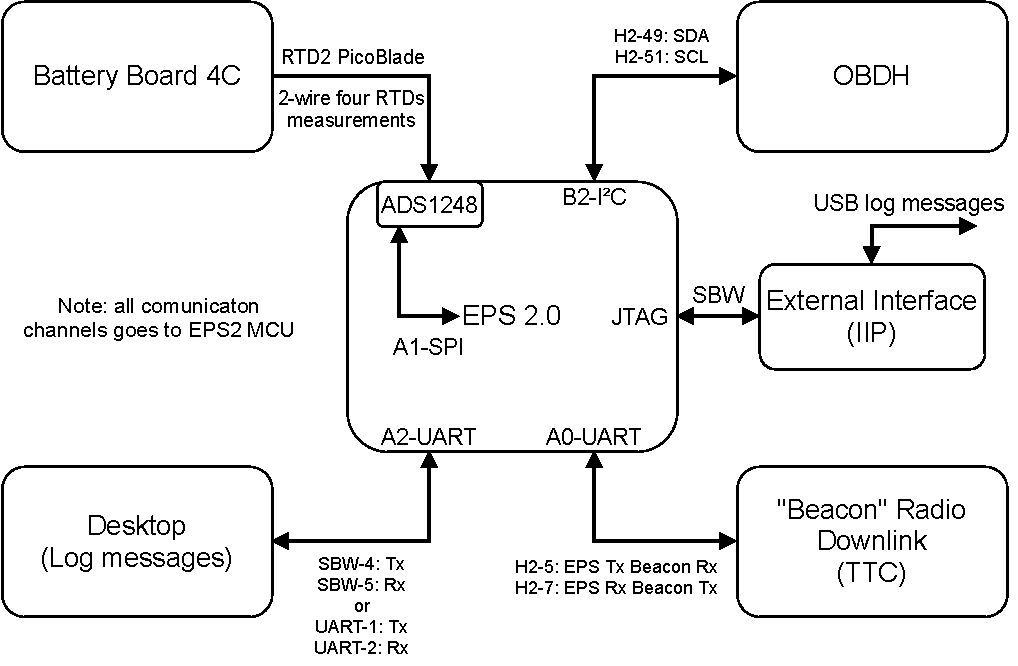
\includegraphics[width=\textwidth]{figures/eps-interfaces-diagram.pdf}
        \caption{EPS interfaces diagram.}
        \label{fig:diagram-interfaces}
    \end{center}
\end{figure}

\begin{table}[!h]
    \centering
    \begin{tabular}{lrrr}
        \toprule[1.5pt]
        \textbf{Peripheral}     & \textbf{USCI} & \textbf{Protocol} & \textbf{Comm. Protocol} \\
        \midrule
        ADS1248                 & A1            & SPI               & - \\
        Beacon Radio            & A0            & UART              & - \\
        PC (log messages)       & A2            & UART              & ANSI messages \\
        DS2777                  & B0            & I$^{2}$C          & - \\
        OBDH                    & B2            & I$^{2}$C          & FSP \\
        External Interface      & -             & JTAG              & Spy-Bi-Wire \\
        \bottomrule[1.5pt]
    \end{tabular}
    \caption{Boards interfaces.}
    \label{tab:interfaces}
\end{table}

\section{Microcontroller}

The MCU consists of a CPU, RAM Memory and Flash Memory (used for program storage and non-volatile status registers). The chosen MCU is a low power 16-bit RISC (\textit{MSP430F6659IPZR}) from Texas Instruments\cite{msp430f6659}. The \autoref{tab:msp430-summary} presents a summary of the main available features and \autoref{fig:msp430-diagram} shows the internal subsystems, descriptions, and peripherals. The microcontroller interfaces, configurations, and auxiliary components are described in the following topics.

\begin{table}[!h]
    \centering
    \begin{tabular}{cllllllll}
        \toprule[1.5pt]
        \textit{Flash} & \textit{SRAM} & \textit{Timers} & \textit{USCI} & \textit{ADC} & \textit{DAC} & \textit{GPIO} \\
        \midrule
        512KB  & 64KB  & 2  & 6 (SPI / I2C / UART)  & 12  & 2  & 74           \\
        \bottomrule[1.5pt]
    \end{tabular}
    \caption{Microcontroller features summary.}
    \label{tab:msp430-summary}
\end{table}

\begin{figure}[!ht]
    \begin{center}
        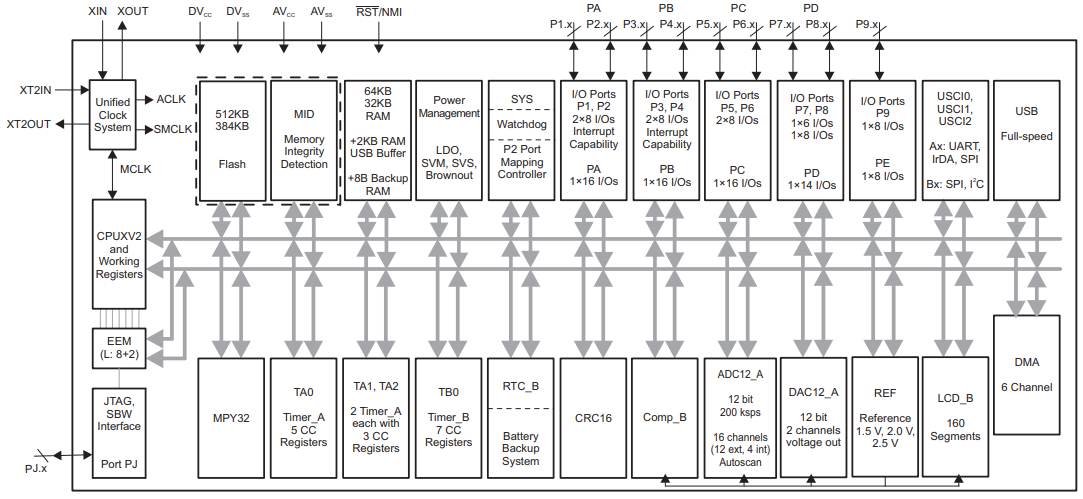
\includegraphics[width=\textwidth]{figures/msp430-diagram.png}
        \caption{Microcontroller internal diagram.}
        \label{fig:msp430-diagram}
    \end{center}
\end{figure}

\subsection{Interfaces Configuration}

The microcontroller has 6 Universal Serial Communication Interfaces (USCI) that can be configured to operate with different protocols and parameters. The \autoref{tab:usci-config} describes each interface configurations.

\begin{table}[!h]
    \centering
    \begin{tabular}{lrrrrl}
        \toprule[1.5pt]
        \textit{Interface} & \textit{Protocol (Index)} & \textit{Mode} & \textit{Word Length} & \textit{Data Rate} & \textit{Configuration} \\
        \midrule
        USCI\_A0           & UART0                     & -             & 8 bits               & 9600 bps           & Stop bits: 1 \\
                           &                           &               &                      &                    & Parity: None \\
        USCI\_A1           & SPI                       & Master        & 8 bits               & TBD                & Phase: High \\
                           &                           &               &                      &                    & Polarity: Low \\
        USCI\_A2           & UART1                     & -             & 8 bits               & 9600 bps           & Stop bits: 1 \\
                           &                           &               &                      &                    & Parity: None \\
        USCI\_B0           & I2C0                      & Master        & 8 bits               & 100 kbps           & Adr. len: 7 bits \\
        USCI\_B2           & I2C1                      & Slave         & 8 bits               & 100 kbps           & Address value: 0x36 \\
        \bottomrule[1.5pt]
    \end{tabular}
    \caption{USCI configuration.}
    \label{tab:usci-config}
\end{table}

\subsection{Voltage Reference}

To generate the 3 volts reference for the MCU internal ADC the EPS uses a \textit{595-REF5025AQDRQ1} chip.
Its circuit schematic can be seen in \autoref{fig:voltage-reference-circuit-schematic} and location on the PCB in \autoref{fig:voltage-reference-circuit-3d}.

\begin{figure}[!ht]
    \begin{center}
        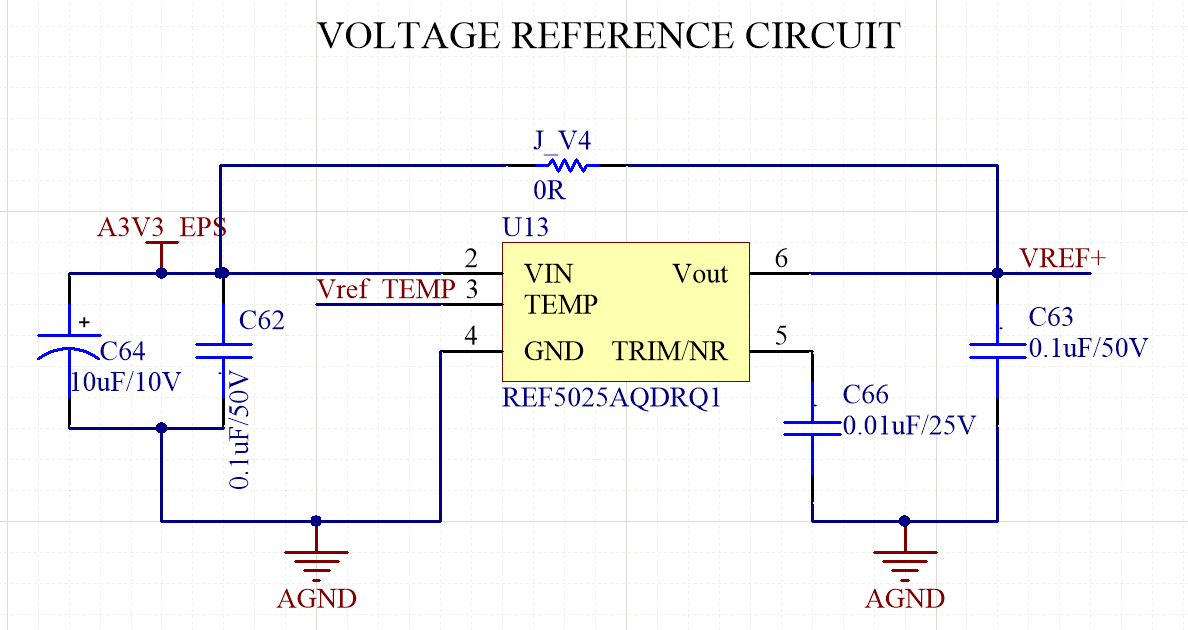
\includegraphics[width=0.8\textwidth]{figures/voltage-reference-circuit-schematic.png}
        \caption{Voltage reference circuit for EPS MCU schematic circuit.}
        \label{fig:voltage-reference-circuit-schematic}
    \end{center}
\end{figure}

\begin{figure}[!ht]
    \begin{center}
        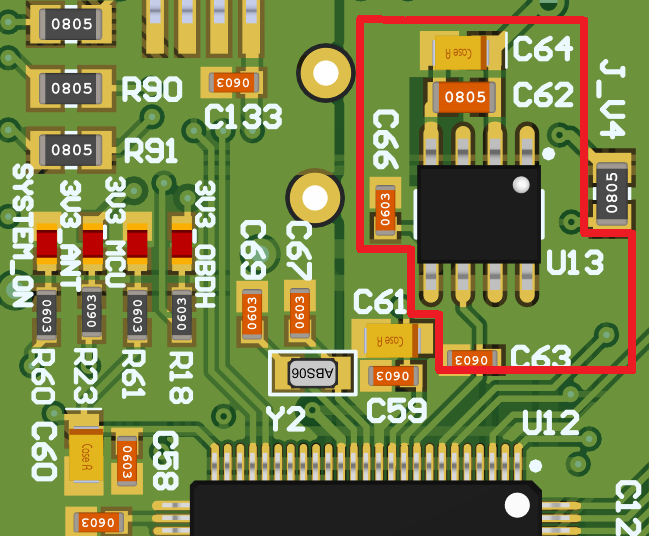
\includegraphics[width=0.5\textwidth]{figures/voltage-reference-circuit-3d.png}
        \caption{Voltage reference circuit for EPS MCU on the PCB.}
        \label{fig:voltage-reference-circuit-3d}
    \end{center}
\end{figure}

\subsection{Clocks Configuration}

Besides the internal clock sources, the microcontroller has two dedicated clock inputs for external crystals: the main clock and the auxiliary clock inputs. There are a 32MHz (\textit{ABM8X-102-32.000MHZ-T}) and a 32.769kHz (\textit{ECS-.327-12.5-34S-TR}) crystals connected to these inputs, respectively. The first source is used for generating the Master Clock (MCLK) and the Subsystem Master Clock (SMCLK), which are used by the CPU and the internal peripheral modules. The second source is used for generating the Auxiliary Clock (ACLK) that handles the low-power modes and might be used for peripherals.


\subsection{Pinout}

An illustration of the microcontroller pinout positions can be seen in the \autoref{fig:msp430-pinout-positions}. The \autoref{tab:mcu-pinout} presents all the EPS 2.0 microcontroller pins assignment.

\begin{figure}[!ht]
    \begin{center}
        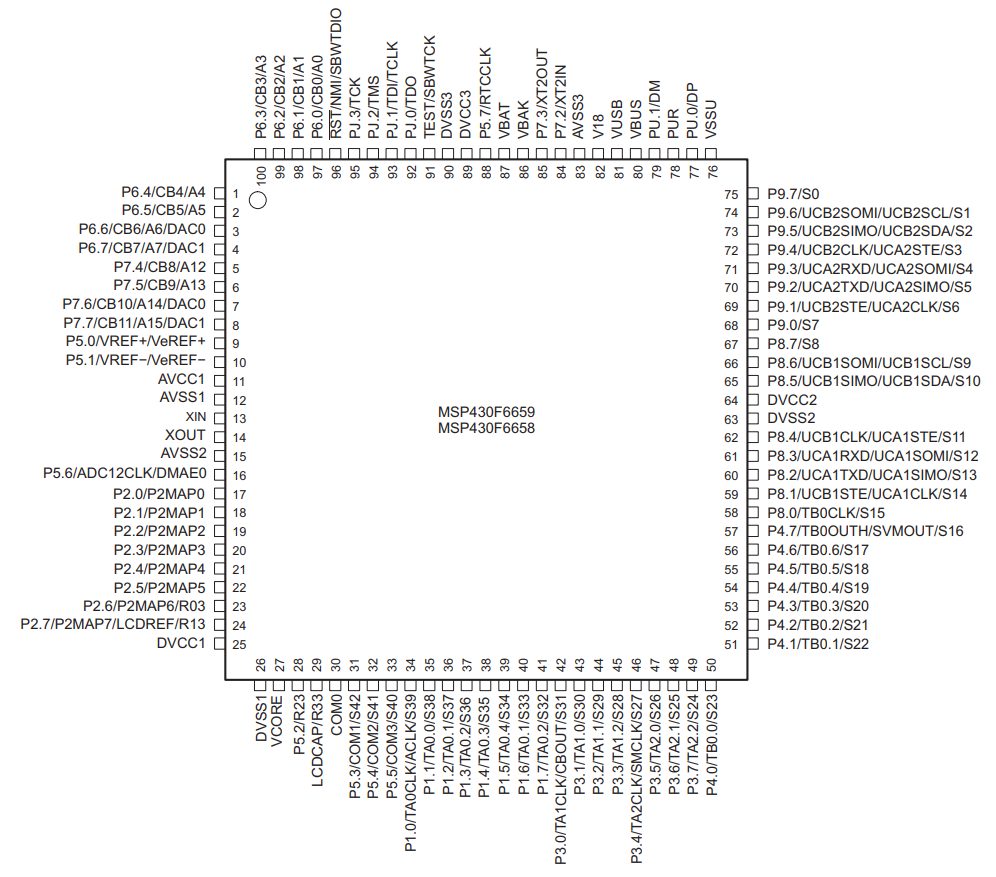
\includegraphics[width=0.9\textwidth]{figures/msp430-pinout.png}
        \caption{Microcontroller pinout positions.}
        \label{fig:msp430-pinout-positions}
    \end{center}
\end{figure}

\begin{longtable}{lcl}
    \toprule[1.5pt]
    \textit{Pin Code} & \textit{Pin Number} & \textit{Signal}       \\
    \midrule
    P1.0              & 34                  & -                 \\
    P1.1              & 35                  & -                 \\
    P1.2              & 36                  & -                 \\
    P1.3              & 37                  & EN\_5V\_PAYLOADS  \\
    P1.4              & 38                  & -             \\
    P1.5              & 39                  & BAT\_GPIO1    \\
    P1.6              & 40                  & BAT\_GPIO2    \\
    P1.7              & 41                  & -             \\
    \midrule
    P2.0              & 17                  & PIO           \\
    P2.1              & 18                  & I2C0\_SDA     \\
    P2.2              & 19                  & I2C0\_SCL     \\
    P2.3              & 20                  & PC104\_GPIO2  \\
    P2.4              & 21                  & UART\_EPS\_TX\_BEACON\_RX     \\
    P2.5              & 22                  & UART\_EPS\_RX\_BEACON\_TX     \\
    P2.6              & 23                  & PC104\_GPIO1                  \\            
    P2.7              & 24                  & PC104\_GPIO0                   \\
    \midrule
    P3.0              & 42                  & -                     \\
    P3.1              & 43                  & -                     \\
    P3.2              & 44                  & HEATER2\_PWM          \\
    P3.3              & 45                  & HEATER1\_PWM          \\
    P3.4              & 46                  & VERSION\_BIT0         \\
    P3.5              & 47                  & VERSION\_BIT1         \\
    P3.6              & 48                  & -                     \\
    P3.7              & 49                  & -                     \\
    \midrule
    P4.0              & 50                  & -                     \\
    P4.1              & 51                  & MPPT\_PWM\_1          \\
    P4.2              & 52                  & MPPT\_PWM\_2          \\
    P4.3              & 53                  & MPPT\_PWM\_3          \\
    P4.4              & 54                  & -                     \\
    P4.5              & 55                  & -                     \\
    P4.6              & 56                  & -                     \\
    P4.7              & 57                  & -                     \\
    \midrule
    P5.0              & 9                   & VREF                  \\
    P5.1              & 10                  & AGND                  \\
    P5.2              & 28                  & -                     \\
    P5.3              & 31                  & SYSTEM\_\_FAULT\_LED  \\
    P5.4              & 32                  & SYSTEM\_ON           \\
    P5.5              & 33                  & -                     \\
    P5.6              & 16                  & -                     \\
    P5.7              & 88                  & -                     \\
    \midrule
    P6.0              & 97                  & ADC1\_$+$Y\_SOLAR\_PANEL\_CURRENT \\
    P6.1              & 98                  & ADC2\_$+$X\_SOLAR\_PANEL\_CURRENT \\
    P6.2              & 99                  & ADC3\_$-$X\_SOLAR\_PANEL\_CURRENT \\
    P6.3              & 100                 & ADC4\_$+$Z\_SOLAR\_PANEL\_CURRENT \\
    P6.4              & 1                   & ADC5\_$-$Z\_SOLAR\_PANEL\_CURRENT \\
    P6.5              & 2                   & ADC6\_$+$Y\_SOLAR\_PANEL\_CURRENT \\
    P6.6              & 3                   & ADC7\_EPS\_TTC\_XCVR\_CURRENT \\
    P6.7              & 4                   & ADC\_MAIN\_POWER\_BUSS\_VOLTAGE \\
    \midrule
    P7.2              & 84                  & XT2\_N                \\
    P7.3              & 85                  & XT2\_P                \\
    P7.4              & 5                   & ADC1\_$-$Y\_$+$X\_SOLAR\_PANEL\_VOLTAGE \\
    P7.5              & 6                   & ADC2\_$-$X\_$+$Z\_SOLAR\_PANEL\_VOLTAGE \\
    P7.6              & 7                   & ADC3\_$-$Z\_$+$Y\_SOLAR\_PANEL\_VOLTAGE \\
    P7.7              & 8                   & ADC\_SOLAR\_PANELS\_TOTAL\_VOLTAGE \\
    \midrule
    P8.0              & 58                  & -                     \\
    P8.1              & 59                  & RTD\_SCLK             \\
    P8.2              & 60                  & RTD\_DIN              \\
    P8.3              & 61                  & RTD\_DOUT             \\
    P8.4              & 62                  & RTD\_RESET            \\
    P8.5              & 65                  & RTD\_CS               \\
    P8.6              & 66                  & RTD\_START            \\
    P8.7              & 67                  & RTD\_DRDY             \\
    \midrule
    P9.0              & 68                  & -                     \\
    P9.1              & 69                  & -                     \\
    P9.2              & 70                  & UART0\_TX             \\
    P9.3              & 71                  & UART0\_RX             \\
    P9.4              & 72                  & I2C1\_EN              \\
    P9.5              & 73                  & I2C1\_SDA             \\
    P9.6              & 74                  & I2C1\_SCL             \\
    P9.7              & 75                  & I2C1\_READY           \\
    \midrule
    PJ.0              & 92                  & -                     \\
    PJ.1              & 93                  & -                     \\
    PJ.2              & 94                  & -                     \\
    PJ.3              & 95                  & -                     \\
    \midrule
    -                 & 13                  & XT1IN                 \\
    -                 & 14                  & XT1OUT                \\
    -                 & 96                  & JTAG\_TDO\_TDI        \\
    -                 & 91                  & JTAG\_TCK             \\
    \bottomrule[1.5pt]
    \caption{Microcontroller pinout and assignments.}
    \label{tab:mcu-pinout}
\end{longtable}

\section{Batteries DaughterBoard}

Due to size restrictions the 4 cell batteries of the EPS2 were allocated to a dauhterboard named Battery Module 4 Cells, a.k.a BAT4C\nomenclature{\textbf{BAT4C}}{\textit{Battery Module 4 Cells.}}\cite{bat4c}. Both boards 3D models are assembled together in a EDA tool as seen in \autoref{fig:eps2-pcb-3d-battery}. BAT4C is connected below EPS2 in a board-to-board connector, the female counterpart (\textit{BAT4CIPS1-105-01-S-D}) present on the EPS is seen in \autoref{fig:battery-connector} with it pinout present on \autoref{tab:battery-connector}. For compability with the older version of the battery module the same connector pads are present near the middle section of the PCB. If the BAT4C is to be used, the connector for these pads must not be soldered, more detail on \autoref{ch:assembly}. Also external connectors are used for temperature measurement and control with RTDs and heaters, more details can be seen on \autoref{rtd-picoblade} and \autoref{heater-picoblade}. 

\begin{figure}[!ht]
    \begin{center}
        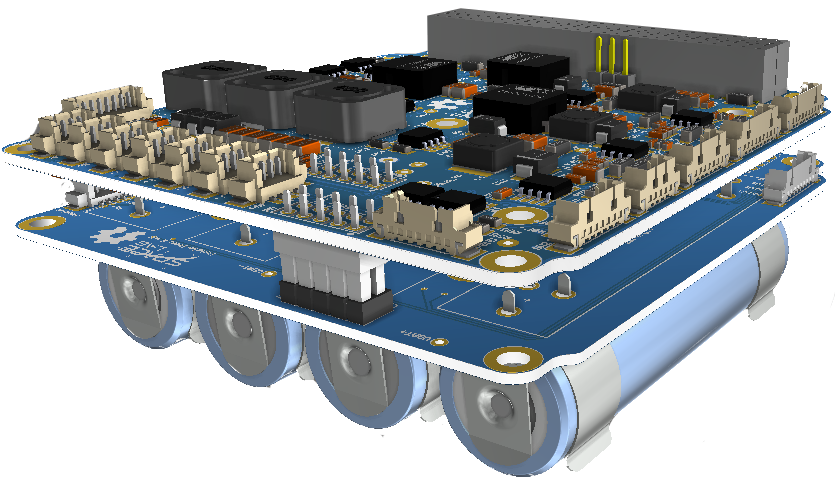
\includegraphics[width=93mm]{figures/eps2-pcb-3d-battery.png}
        \caption{EPS2 and BAT4C 3D models assembled.}
        \label{fig:eps2-pcb-3d-battery}
    \end{center}
\end{figure}

\begin{figure}[!ht]
    \begin{center}
        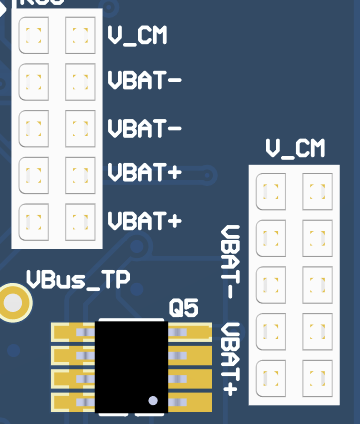
\includegraphics[width=0.35\textwidth]{figures/battery-connector.png}
        \caption{EPS2 battery connectors.}
        \label{fig:battery-connector}
    \end{center}
\end{figure}

\begin{table}[!h]
    \centering
    \begin{tabular}{cllll}
        \toprule[1.5pt]
        \textit{Pin} & \textit{Row} \\
        \midrule
        1            & $+$Vbat \\
        2            & $+$Vbat \\
        3            & $+$Vbat \\
        4            & $+$Vbat \\
        5            & $-$Vbat \\
        6            & $-$Vbat \\
        7            & $-$Vbat \\
        8            & $-$Vbat \\
        9            & Vbat\_Common \\
        10           & Vbat\_Common \\
        \bottomrule[1.5pt]
    \end{tabular}
    \caption{Battery connector pinout.}
    \label{tab:battery-connector}
\end{table}

\section{Solar Panels}

The energy harvesting system is based on solar energy conversion through ten solar panels attached to a 2U CubeSat structure. The solar panels are connected through six 4 pin PicoBlade connectors \textit{0533980471}. Because the EPS2 module has only six input connectors four pairs of solar panels will be connected in paralel. The connection scheme of the solar panels is visible in \autoref{fig:diagram-solar-panels}. The input connectors for the solar panels power are described in \autoref{solar-panels-picoblades}.
\begin{figure}[!ht]
    \begin{center}
        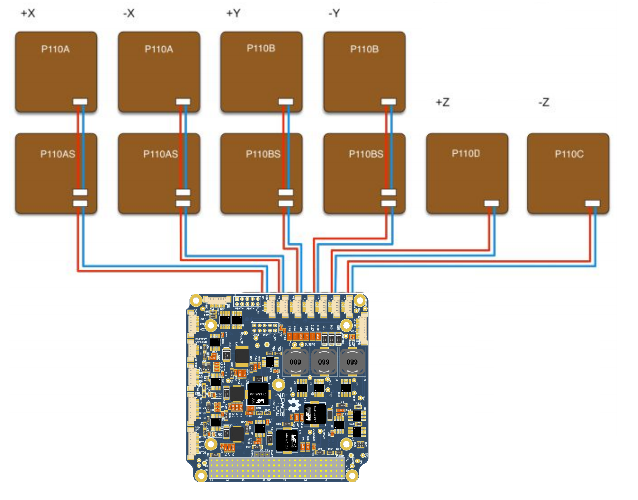
\includegraphics[width=0.75\textwidth]{figures/diagram-solar-panels.png}
        \caption{Solar panels connection to EPS2.}
        \label{fig:diagram-solar-panels}
    \end{center}
\end{figure}

\section{I2C Buffer}

The microcontroller I2C interface have a dedicated IC buffer, which improve the signal quality throughout the various connectors and offers reliability enhancements, since it protects the bus in case of failures. This measure was adopted in all the satellite modules due to previous failures in I2C buses. Using this scheme, the modules connected though this protocol might have shared connections without losing performance or reliability. 

The buffer selected for this function is the Texas Instruments \textit{TCA4311}. Besides the I2C inputs and outputs, it features control and status signals that are connected to GPIOs in the microcontroller: an enable and an operation ready status. Also, both inputs and outputs in these I2C lines have external pull-up resistors. Its circuit schematic can be see \autoref{fig:i2c-buffer-circuit}.

\begin{figure}[!ht]
    \begin{center}
        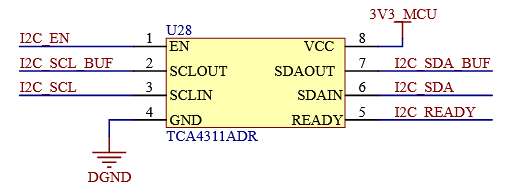
\includegraphics[width=0.65\textwidth]{figures/i2c-buffer-circuit.png}
        \caption{I2C buffer circuit.}
        \label{fig:i2c-buffer-circuit}
    \end{center}
\end{figure}

\section{MPPT Subsystem}

On the MPPT subsystem the main components are the MPPT boost converters, solar panels voltage and current sensors. These measurement circuits are used to generate a voltage proportional to the variable being measured, in a range accepted by the MCU internal ADC.

\subsection{MPPT Boost Converters}

There are three boost converters in the system, one for each couple of solar panels in parallel connection. Each one is a discrete boost with a \textit{HC9-220-R} inductor, a \textit{SI4166DY} mosfet as the switch and a \textit{B340LA-13-F} diode. There are six \textit{GRM32ER1E226KE15L} capacitors and two \textit{GRM216R71H103KA01D} capacitors connected in parallel in the boost output. The output filter is the same for all the converters as their outputs are tied together. The control PWM signals are generated by the MCU at a frequency of nearly 500 kHz.
One of the MPPT boosters circuit schematic can be seen in \autoref{fig:mppt-boosters-circuit-schematic} and location of all three at the PCB in \autoref{fig:mppt-boosters-circuit-3d}.

\begin{figure}[!ht]
    \begin{center}
        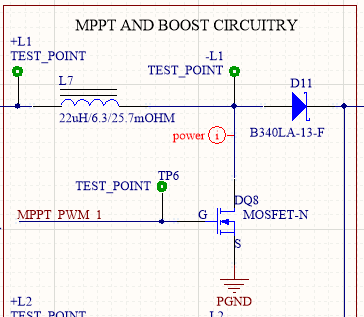
\includegraphics[width=0.5\textwidth]{figures/mppt-boosters-circuit-schematic.png}
        \caption{One of the MPPT boosters schematic circuit.}
        \label{fig:mppt-boosters-circuit-schematic}
    \end{center}
\end{figure}

\begin{figure}[!ht]
    \begin{center}
        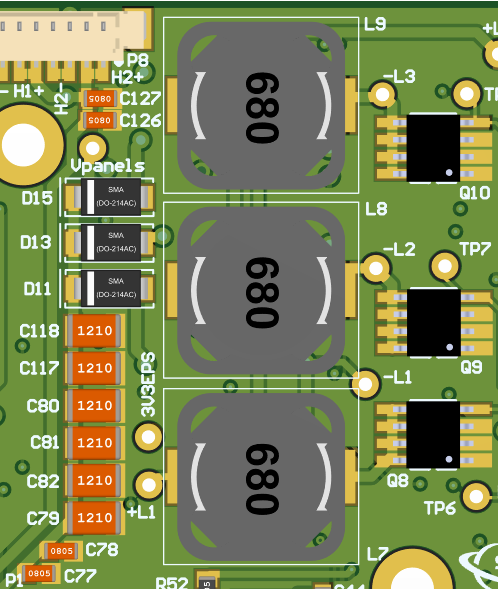
\includegraphics[width=0.5\textwidth]{figures/mppt-boosters-circuit-3d.png}
        \caption{MPPT boost converters circuit on the PCB.}
        \label{fig:mppt-boosters-circuit-3d}
    \end{center}
\end{figure}

\subsection{Solar Panels Current}

The main component of the solar panels currents measurement circuit is the \textit{MAX9934TAUA+} current sense amplifier. It generates an output current proportional to the differential input voltage. The gain is 25 $\mu$A/mV. It was considered a maximum current load sourced by two solar panels in parallel on the most optimist scenario of 1.5 A . To make the measurements possible, the current goes through 20 m$\Omega$, 0.5 \% resistors, connected to the inputs of the amplifier, and the outputs are connected to 3.3 k$\Omega$ resistors. The output voltage of the circuit is given by:

\begin{equation}
V_{out} = I_{load} \cdot R_{sense} \cdot G_{m} \cdot R_{out}
\end{equation}

The voltage drop in $R_{sense}$ generates a proportional $I_{out}$ on the IC of approximately 750 $\mu$A.
In total there are six of these current measurement circuits for the six sides of the CubeSat.
Two of the inputs of the solar panels circuit schematic can be seen in \autoref{fig:solar-panels-current-circuit-schematic} and location of all six at the PCB in \autoref{fig:solar-panels-current-circuit-3d}.

\begin{figure}[!ht]
    \begin{center}
        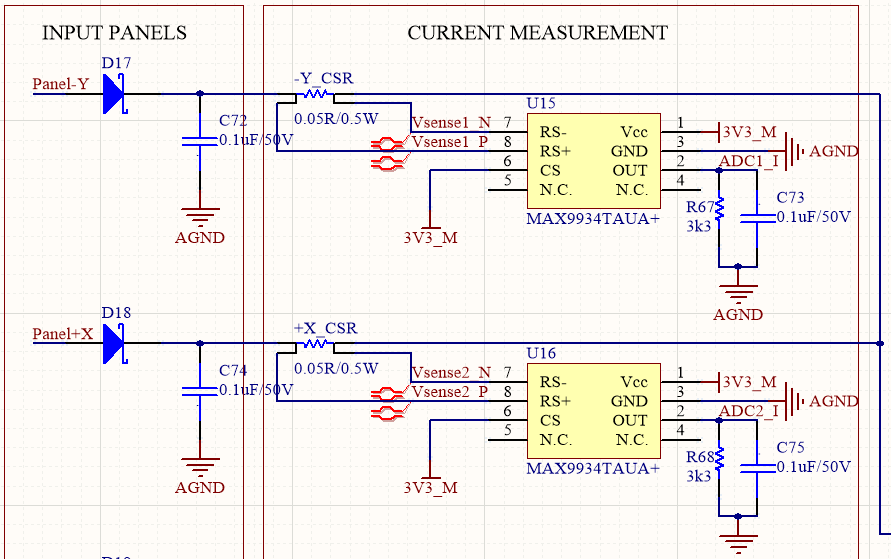
\includegraphics[width=0.85\textwidth]{figures/solar-panels-current-circuit-schematic.png}
        \caption{Solar panels $-$Y and $+$X input circuit schematic.}
        \label{fig:solar-panels-current-circuit-schematic}
    \end{center}
\end{figure}

\begin{figure}[!ht]
    \begin{center}
        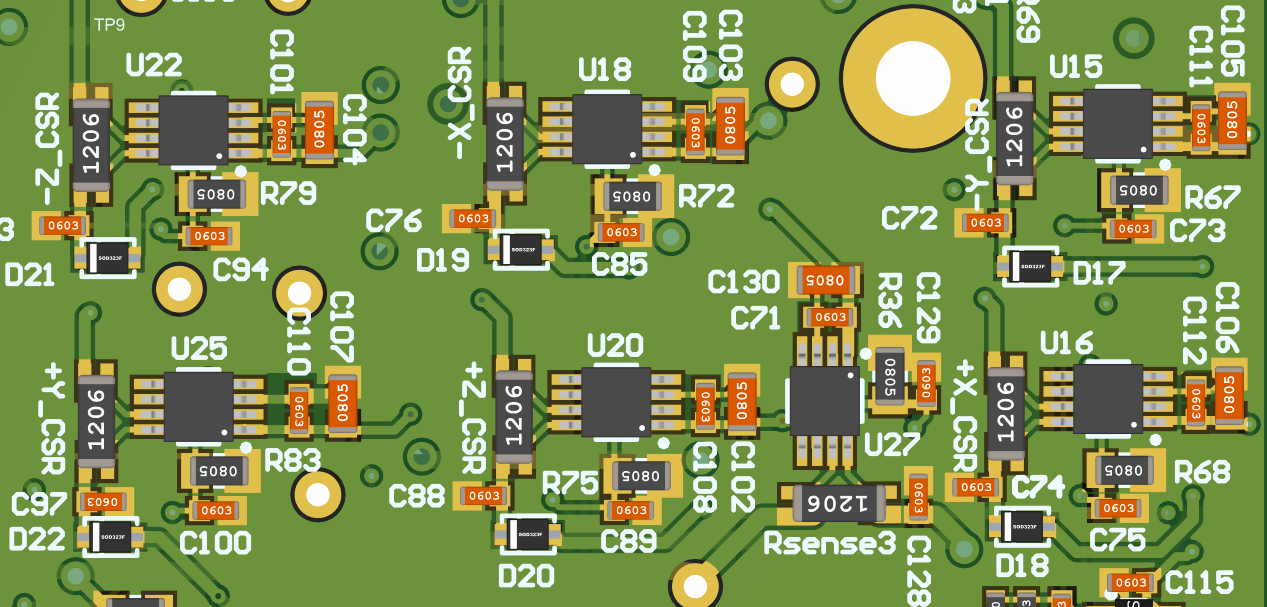
\includegraphics[width=0.85\textwidth]{figures/solar-panels-current-circuit-3d.png}
        \caption{Solar panels current measurement circuits on the PCB.}
        \label{fig:solar-panels-current-circuit-3d}
    \end{center}
\end{figure}


\subsection{Solar Panels Voltage}

The solar panels voltage measurement circuit is composed by a voltage divider and an op-amp in a buffer configuration. The voltage divider is composed of a 93.1 k$\Omega$ resistor and an 100 k$\Omega$ resistor. The op-amp is a \textit{TLV341AIDBVR} chip. The output voltage is given by:

\begin{equation}
V_{out} = V_{sp} \cdot \frac{R_{2}}{R_{1} + R_{2}}
\end{equation}

In total there are three of these voltage measurement circuits, the solar panels sides that are meassured together are: $-$Y with $+$X, $-$X with $+$Z and $-$Z with $+$Y.
One of the voltage measurement circuit schematic can be seen in \autoref{fig:solar-panels-voltage-circuit-schematic}.

\begin{figure}[!ht]
    \begin{center}
        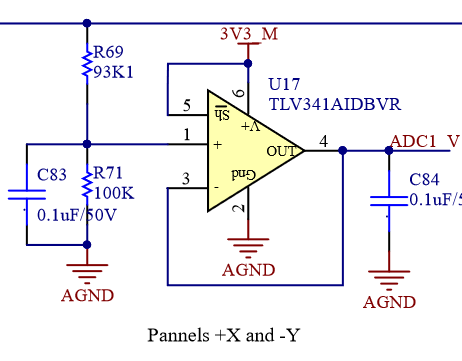
\includegraphics[width=0.5\textwidth]{figures/solar-panels-voltage-circuit-schematic}
        \caption{Solar panels $-$Y and $+$X voltage measurement circuit schematic.}
        \label{fig:solar-panels-voltage-circuit-schematic}
    \end{center}
\end{figure}

\section{Batteries Managment Subsystem}

On the batteries managment subsystem the main components are the battery control circuit, external ADC chip, solar panels and batteries kill-switches, heater drivers and voltage sensors for the boosters output and main power bus. 

\subsection{Boost Converters Output Voltage}

The boost converters output voltage measurement circuit is very similar to the solar panels voltages measurement circuit, with the exception that the voltage divider is composed by a 300 k$\Omega$ resistor and an 100 k$\Omega$ resistor.
The schematic for the voltage measurement circuit of the solar panels can be seen again for reference in \autoref{fig:solar-panels-voltage-circuit-schematic}.

\subsection{Kill-Switches and Remove Before Flight}

These switches are used to separate the solar panels and the batteries from the load during pre-flight and launch. Each one is composed of two \textit{SI4403-CDY-T1-GE3} P-channel mosfets in parallel, as a redundancy.
The Kill-Switches and RBF\nomenclature{\textbf{RBF}}{\textit{Remove Before Flight.}} are interfaced on the EPS board via external PicoBlade cables to its respective external mechanisms. RBF functions by simply short circuting the pins of the pin header present on an external interface\cite{iip}, and for the kill-switches it is required to press the spring buttons on the CubeSat structure, this is naturally done when the nanosatellite in integrated into the deployer.
On \autoref{kill-switches-picoblades} and \autoref{rbf-picoblade} it is showed the pinouts and locations for these connectors.

\subsection{Battery Control Circuit}

The batteries are monitored by the \textit{DS2777} chip. It measures several parameters and sends them to the EPS2 MCU via I2C protocol. The factory default value for its slave address is 0x59. Also it automatically protects the batteries against short-circuits, overvoltage and undervoltage situations by switching two \textit{FDS6898AZ} mosfets.
Its circuit schematic can be seen in \autoref{fig:bms-circuit-schematic} and location on the PCB in \autoref{fig:bms-circuit-3d}.

\begin{figure}[!ht]
    \begin{center}
        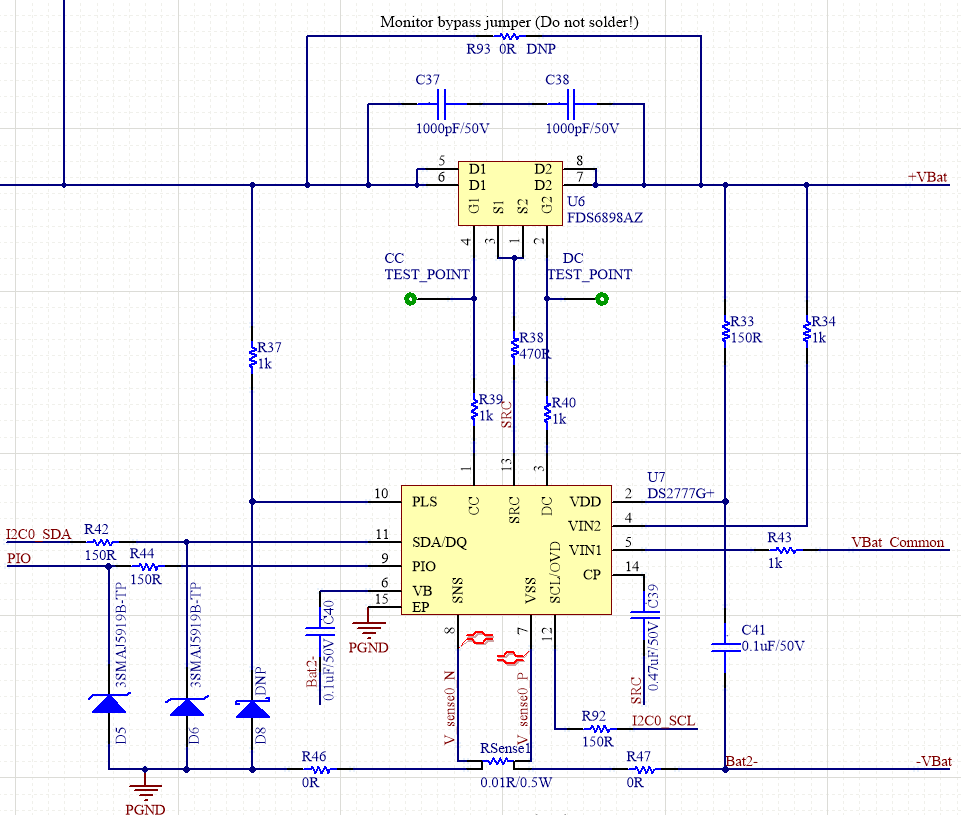
\includegraphics[width=0.85\textwidth]{figures/bms-circuit-schematic.png}
        \caption{Battery monitor circuit schematic.}
        \label{fig:bms-circuit-schematic}
    \end{center}
\end{figure}

\begin{figure}[!ht]
    \begin{center}
        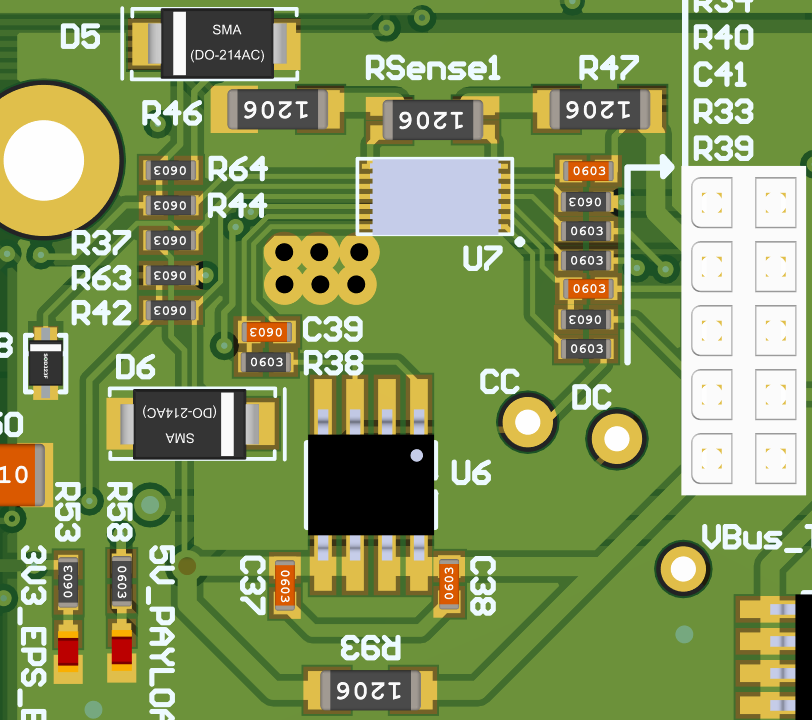
\includegraphics[width=0.5\textwidth]{figures/bms-circuit-3d.png}
        \caption{Battery monitor circuit on the PCB.}
        \label{fig:bms-circuit-3d}
    \end{center}
\end{figure}

\subsection{Main Power Bus Voltage}

The main power bus voltage measurement circuit is identical to the boost converters output voltage measurement circuit.
The schematic for the voltage measurement circuit of the solar panels can be seen again for reference in \autoref{fig:solar-panels-voltage-circuit-schematic}.

\subsection{External ADC}

The \textit{ADS1248} chip generates a precise reference current to the RTDs, and samples the voltage proportional to the temperature established over the sensors. This voltage is converted to digital data and sent to the MCU via SPI protocol.
The location the IC and its subcircuitry can be seen in \autoref{fig:ads1248-circuit-3d}.

\begin{figure}[!ht]
    \begin{center}
        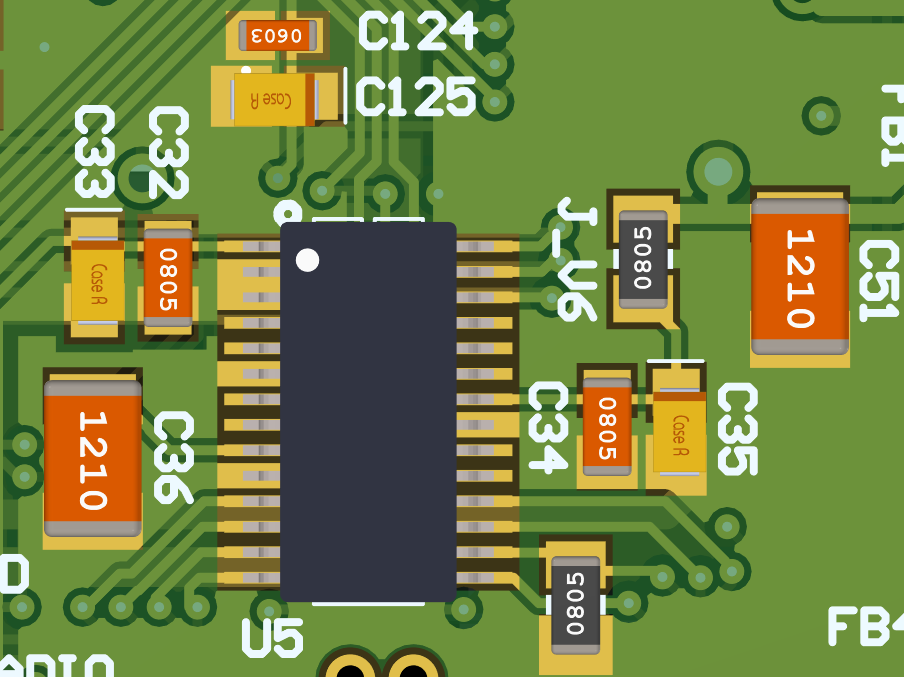
\includegraphics[width=0.5\textwidth]{figures/ads1248-circuit-3d.png}
        \caption{ADS1248 circuit on the PCB.}
        \label{fig:ads1248-circuit-3d}
    \end{center}
\end{figure}

\subsection{Heaters Drivers}

The drivers are chopper converters controlled by the MCU, with a PWM frequency of 50 kHz. The switches of the chopper converters are \textit{Si4010DY} mosfets.
Its circuit schematic can be seen in \autoref{fig:heaters-circuit-schematic} and location on the PCB in \autoref{fig:heaters-drivers-circuit-3d}.

\begin{figure}[!ht]
    \begin{center}
        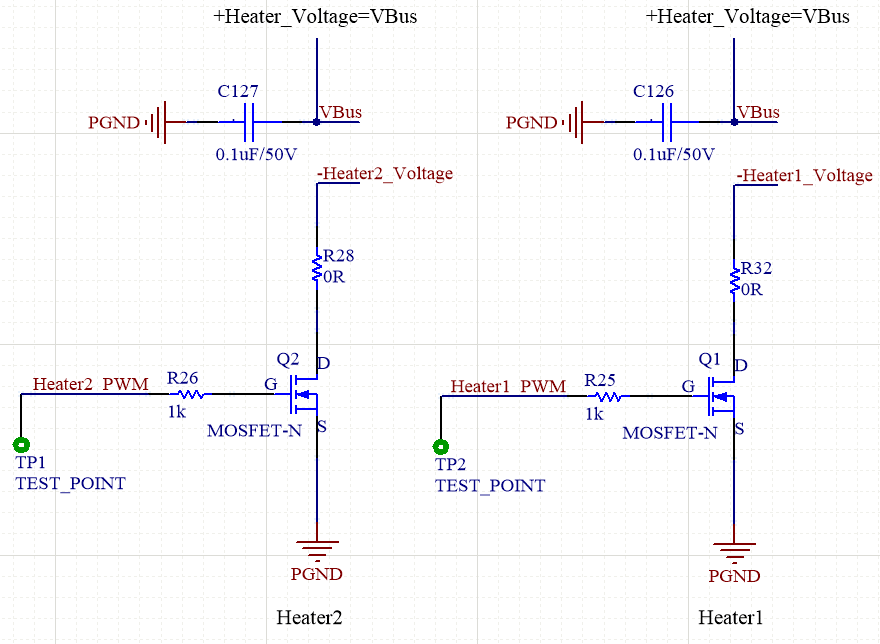
\includegraphics[width=0.85\textwidth]{figures/heaters-drivers-circuit-schematic.png}
        \caption{Hearter drivers circuit schematic.}
        \label{fig:heaters-circuit-schematic}
    \end{center}
\end{figure}

\begin{figure}[!ht]
    \begin{center}
        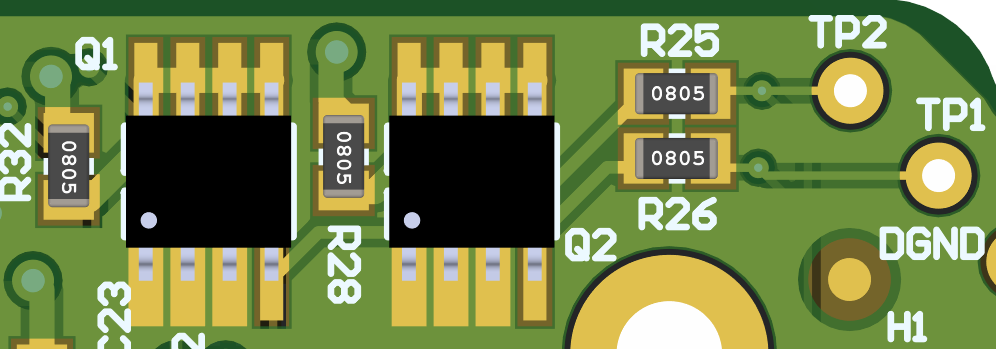
\includegraphics[width=0.5\textwidth]{figures/heaters-drivers-circuit-3d.png}
        \caption{Hearter drivers circuit on the PCB.}
        \label{fig:heaters-drivers-circuit-3d}
    \end{center}
\end{figure}

\section{Power Converters Subsystem}

The EPS2 has 6 integrated buck DC-DC regulators, all these are powered from the main power bus. Some regulators are always enabled, others are can be enabled or disabled by the EPS2 or other module.

\subsection{EPS/TTC Regulator}

To supply the TTC MCU (also called "Beacon MCU") and EPS2 MCU and its subcircuits a \textit{TPS5420QDRQ1} regulator is used, with and output voltage of 3.3 V and 2 A current capability. This regulator is always on.
The EPS/TTC circuit location on the PCB can be seen in \autoref{fig:eps-beacon-buck-circuit-3d}.

\begin{figure}[!ht]
    \begin{center}
        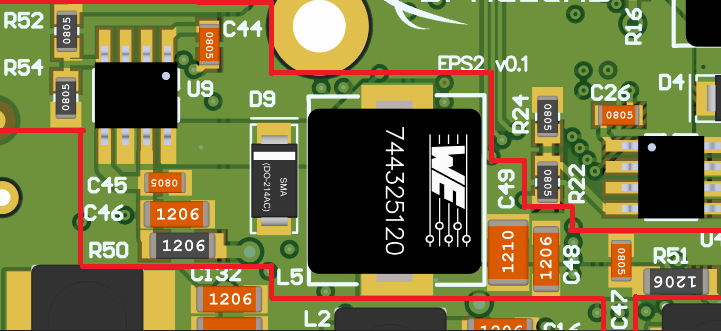
\includegraphics[width=0.5\textwidth]{figures/eps-beacon-buck-circuit-3d.png}
        \caption{EPS/TTC regulator circuit on the PCB.}
        \label{fig:eps-beacon-buck-circuit-3d}
    \end{center}
\end{figure}

There is also a current measurement at the output of the EPS/TTC regulator. It also uses a \textit{MAX9934TAUA+} current sense amplifier, but with a shunt resistor of 75 m$\Omega$, 0.5 \% and the output connected to a 4.02 k$\Omega$ resistor.
The circuit schematic is almost the same as \autoref{fig:solar-panels-current-circuit-schematic} only changing the resistors and capacitor values, its location on the PCB is the labeled U27 IC and its passive components in \autoref{fig:solar-panels-current-circuit-3d}.

\subsection{OBDH Regulator}

The OBDH is powered by a \textit{TPS5410QDRQ1} regulator, with an output voltage of 3.3 V and 1 A current capability.
Its location on the PCB can be seen in \autoref{fig:obdh-buck-circuit-3d}.

\begin{figure}[!ht]
    \begin{center}
        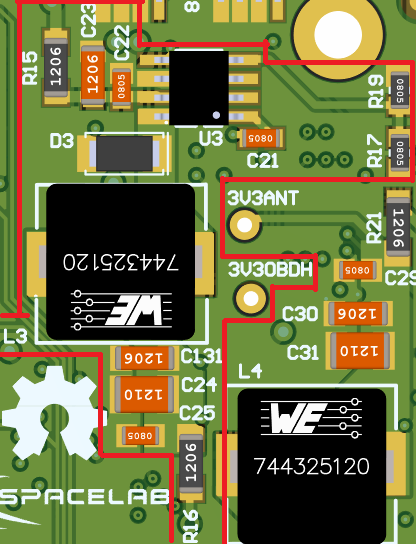
\includegraphics[width=0.3\textwidth]{figures/obdh-buck-circuit-3d.png}
        \caption{OBDH regulator circuit on the PCB.}
        \label{fig:obdh-buck-circuit-3d}
    \end{center}
\end{figure}

\subsection{Antenna Deployer Regulator}

The antenna deployment system has a dedicated regulator \textit{TPS5420QDRQ1}, with 3.3 V output voltage and 2 A current capability. This regulator is always on.
Its location on the PCB can be seen in \autoref{fig:ant-buck-circuit-3d}.

\begin{figure}[!ht]
    \begin{center}
        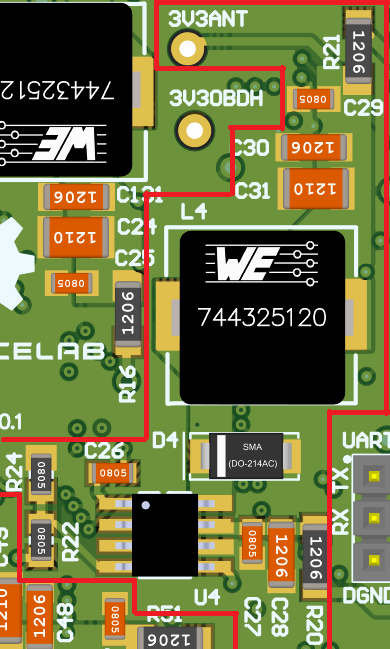
\includegraphics[width=0.3\textwidth]{figures/ant-buck-circuit-3d.png}
        \caption{Antenna deployer regulator circuit on the PCB.}
        \label{fig:ant-buck-circuit-3d}
    \end{center}
\end{figure}

\subsection{Radio 0 Transceiver Regulator}

The radio 0 XCVR\nomenclature{\textbf{XCVR}}{\textit{Transceiver.}} responsible for the Downlink/Uplink of the CubeSat is powered by a \textit{TPS54540QDDARQ1} regulator, with an output voltage of 5V and 5A campability. The OBDH can enable/disable this regulator.
Its location on the PCB can be seen in \autoref{fig:main-radio-buck-circuit-3d}.

\begin{figure}[!ht]
    \begin{center}
        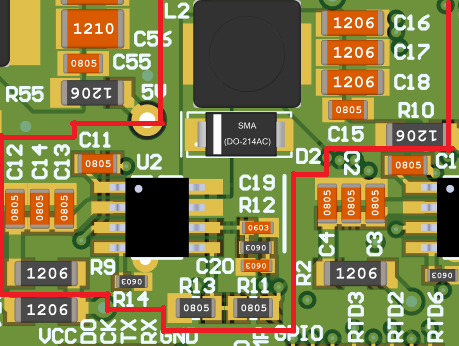
\includegraphics[width=0.5\textwidth]{figures/main-radio-buck-circuit-3d.png}
        \caption{Main radio transceiver regulator circuit on the PCB.}
        \label{fig:main-radio-buck-circuit-3d}
    \end{center}
\end{figure}

\subsection{Radio 1 Transceiver Regulator}

The radio 1 XCVR responsible for a periodic data sent status of the CubeSat is powered by a \textit{TPS54540QDDARQ1} regulator, with 6V output voltage and 5A campability. The Beacon MCU can enable/disable this regulator.
Its location on the PCB can be seen in \autoref{fig:beacon-radio-buck-circuit-3d}.

\begin{figure}[!ht]
    \begin{center}
        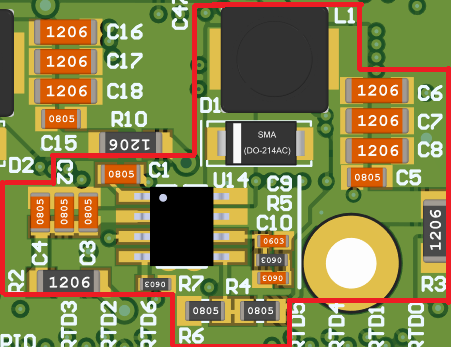
\includegraphics[width=0.5\textwidth]{figures/beacon-radio-buck-circuit-3d.png}
        \caption{Beacon radio transceiver regulator circuit on the PCB.}
        \label{fig:beacon-radio-buck-circuit-3d}
    \end{center}
\end{figure}

\subsection{Payloads Regulator}

To power the payloads a \textit{TPS5430QDDARQ1} regulator is used. It has an output voltage of 5 V and 3 A current capability. The EPS2 can enable/disable this regulator.
Its location on the PCB can be seen in \autoref{fig:payloads-buck-circuit-3d}.

\begin{figure}[!ht]
    \begin{center}
        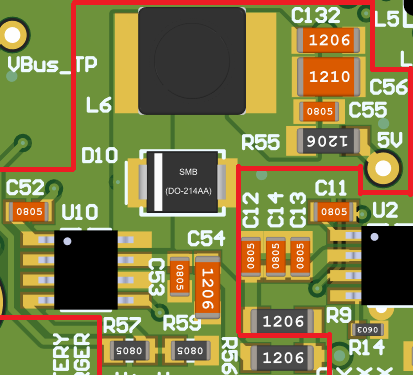
\includegraphics[width=0.5\textwidth]{figures/payloads-buck-circuit-3d.png}
        \caption{Payloads regulator circuit on the PCB.}
        \label{fig:payloads-buck-circuit-3d}
    \end{center}
\end{figure}

\section{External Connectors} \label{external-connectors}

The EPS2 module is connected to the other modules using the PC104 bus. The solar panels, the kill-switches, the remove before flight, the RTDs, the heater, the batteries charger connector and the JTAG pins are connected using Molex PicoBlade connectors. The EPS2 module also has a jumper that connects the MCU VCC to the JTAG VCC and a header to debug the board via UART protocol. In the following sections each connector is detailed, with a picture showing the location on the EPS2 PCB and a table explaining each pin function.

\subsection{PC104} \label{PC104}

The connector referred as PC-104 is a junction of two double row 28H headers (\textit{SSW-126-01-G-D}). These connectors create a solid 104-pin interconnection across the different satellite modules. The \autoref{fig:pc104-scheme} shows the PC-104 interface from the bottom side of the PCB, which allows visualize the simplified label scheme in the board. Also, the \autoref{tab:pc104-pins} provides the connector pinout\footnote{This pinout is simplified since additional interfaces were omitted. Refer to \textit{option sheet} in chapter \ref{ch:assembly}.} for the pins that are connected to the module. 

\begin{figure}[!ht]
    \begin{center}
        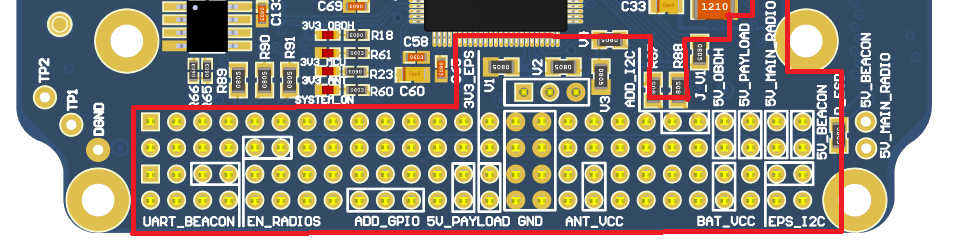
\includegraphics[width=0.8\textwidth]{figures/eps2_pc104_scheme.png}
        \caption{Bottom view of PC-104 and simplified labels.}
        \label{fig:pc104-scheme}
    \end{center}
\end{figure}

\begin{table}[!h]
    \centering
    \begin{tabular}{cllll}
        \toprule[1.5pt]
        \textit{Pin [A-B]} & \textit{H1A}     & \textit{H1B}     & \textit{H2A}  & \textit{H2B}  \\
        \midrule
        1-2                & -                & -                & -             & -             \\
        3-4                & -                & -                & -             & -             \\
        5-6                & -                & -                & UART\_RX      & -             \\
        7-8                & -                & -                & UART\_TX      & -             \\
        9-10               & -                & EN\_PWR\_5       & -             & -             \\
        11-12              & -                & EN\_PWR\_6       & -             & -             \\
        13-14              & -                & -                & -             & -             \\
        15-16              & -                & -                & -             & -             \\
        17-18              & -                & -                & -             & -             \\
        19-20              & -                & -                & -             & -             \\
        21-22              & -                & -                & -             & -             \\
        23-24              & -                & -                & -             & -             \\
        25-26              & -                & -                & PWR\_4\_5V    & PWR\_4\_5V    \\
        27-28              & -                & -                & PWR\_7\_3V3   & PWR\_7\_3V3   \\
        29-30              & GND              & GND              & GND           & GND           \\
        31-32              & GND              & GND              & GND           & GND           \\
        33-34              & -                & -                & -             & -             \\
        35-36              & -                & -                & PWR\_1\_3V3   & PWR\_1\_3V3   \\
        37-38              & -                & -                & -             & -             \\
        39-40              & -                & -                & -             & -             \\
        41-42              & -                & -                & -             & -             \\
        43-44              & -                & -                & -             & -             \\
        45-46              & PWR\_2\_3V3      & PWR\_2\_3V3      & PWR\_3\_BAT   & PWR\_3\_BAT   \\
        47-48              & PWR\_4\_5V       & PWR\_4\_5V       & -             & -             \\
        49-50              & PWR\_5\_5V       & PWR\_5\_5V       & I2C\_SDA      & -             \\
        51-52              & PWR\_6\_6V       & PWR\_6\_6V       & I2C\_SCL      & -             \\
        \bottomrule[1.5pt]
    \end{tabular}
    \caption{PC-104 connector pinout.}
    \label{tab:pc104-pins}
\end{table}

\begin{table}[!h]
    \centering
    \begin{tabular}{lL{0.29\textwidth}L{0.47\textwidth}}
        \toprule[1.5pt]
        \textbf{Signal}  & \textbf{Pin(s)}            & \textbf{Description} \\
        \midrule
        GND              & H1-29, H1-30, H1-31, H1-32, H2-29, H2-30, H2-31, H2-32 & Ground reference \\
        PWR\_1\_3V3      & H2-35, H2-36               & Power bus 1, 3.3 V, 2 A max. \\
        PWR\_2\_3V3      & H1-45, H1-46               & Power bus 2, 3.3 V, 1 A max. \\
        PWR\_3\_BAT      & H2-45, H2-46               & Power bus 3, battery terminals (+) \\
        PWR\_4\_5V       & H1-47, H1-48, H2-25, H2-26 & Power bus 4, 5 V, 3 A max. \\
        PWR\_5\_5V       & H1-49, H1-50               & Power bus 5, 5 V, 5 A max. \\
        PWR\_6\_6V       & H1-51, H1-52               & Power bus 6, 6 V, 5 A max. \\
        PWR\_7\_3V3      & H2-27, H2-28               & Power bus 7, 3.3 V, 2 A max. \\
        I2C\_SDA         & H2-49                      & Primary communication bus (data signal) \\
        I2C\_SCL         & H2-51                      & Primary communication bus (clock signal) \\
        UART\_RX         & H2-5                       & Secondary communication bus (RX) \\
        UART\_TX         & H2-7                       & Secondary communication bus (TX) \\
        EN\_PWR\_5       & H1-10                      & Enable signal of the power bus 5 \\
        EN\_PWR\_6       & H1-12                      & Enable signal of the power bus 6 \\
        \bottomrule[1.5pt]
    \end{tabular}
    \caption{PC-104 bus signal description.}
    \label{tab:pc104-signals}
\end{table}

\subsection{Solar Panels PicoBlades} \label{solar-panels-picoblades}

There are six PicoBlade connectors that can be connected to solar panels. Each one of them is to be used with its respective positive or negative cartesian axis reference label: X, Y or Z. Note that the total current for each individual PicoBlade pin must not exceed 1000mA, this means that the maximum current per connector is 2000mA.
Their pinout is showed in \autoref{tab:solar-panels-picoblades} and position on the PCB in \autoref{fig:solar-panels-picoblades}.

\begin{table}[!h]
    \centering
    \begin{tabular}{cl}
        \toprule[1.5pt]
        \textit{Pin} & \textit{Row} \\
        \midrule
        1            & Panel [side reference] positive input\\
        2            & Panel [side reference] positive input \\
        3            & PGND \\
        4            & PGND \\
        \bottomrule[1.5pt]
    \end{tabular}
    \caption{Solar panels PicoBlades pinout.}
    \label{tab:solar-panels-picoblades}
\end{table}

\begin{figure}[!ht]
    \begin{center}
        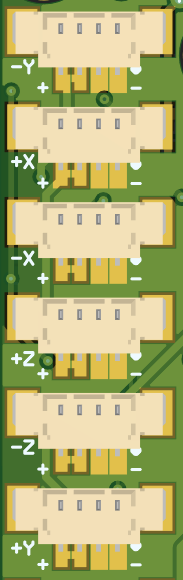
\includegraphics[width=0.2\textwidth]{figures/solar-panels-picoblades-3d.png}
        \caption{Solar panels power input connectors on the PCB.}
        \label{fig:solar-panels-picoblades}
    \end{center}
\end{figure}

\subsection{Kill-Switches PicoBlades} \label{kill-switches-picoblades}

There are two PicoBlade connectors to be connected to two separete kill-switch spring button mechanisms, one of the mechanism is ilustrated in \autoref{fig:kill-switch-installed}. The connection is done by manually soldering and isolating with a heat shrink tube, the other end of the cable goes to PicoBlades of the EPS, their pinout is showed in \autoref{tab:kill-switches-picoblades} and position on the PCB in \autoref{fig:kill-switches-picoblades}.

\begin{figure}[!ht]
    \begin{center}
        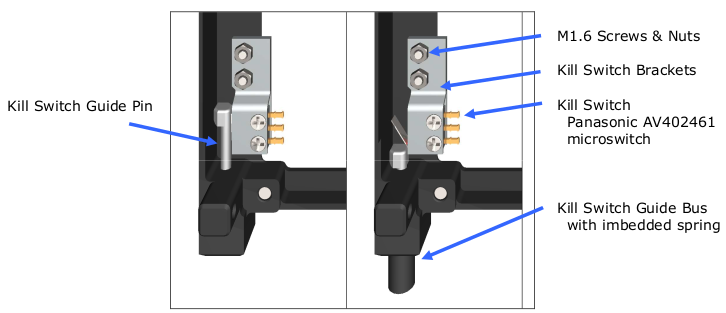
\includegraphics[width=\textwidth]{figures/kill-switch-installed.png}
        \caption{Kill-switch spring button mechanism.}
        \label{fig:kill-switch-installed}
    \end{center}
\end{figure}

\begin{table}[!h]
    \centering
    \begin{tabular}{cl}
        \toprule[1.5pt]
        \textit{Pin} & \textit{Row} \\
        \midrule
        1            & Common \\
        2            & Common \\
        3            & NO\nomenclature{\textbf{NO}}{\textit{Normally open.}} \\
        4            & NO\nomenclature{\textbf{NO}}{\textit{Normally open.}} \\
        5            & NC\nomenclature{\textbf{NC}}{\textit{Normally closed.}} \\
        6            & NC\nomenclature{\textbf{NC}}{\textit{Normally closed.}} \\
        \bottomrule[1.5pt]
    \end{tabular}
    \caption{Kill-switches PicoBlades pinout.}
    \label{tab:kill-switches-picoblades}
\end{table}

\begin{figure}[!ht]
    \begin{center}
        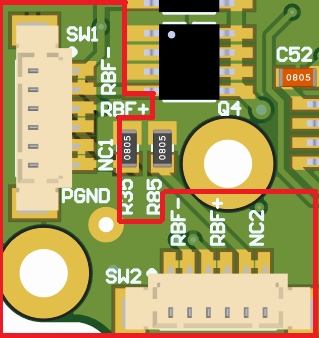
\includegraphics[width=0.35\textwidth]{figures/kill-switches-picoblades-3d.png}
        \caption{Kill-switches PicoBlade connectors on the PCB.}
        \label{fig:kill-switches-picoblades}
    \end{center}
\end{figure}

\subsection{RBF PicoBlade} \label{rbf-picoblade}

The RBF PicoBlade interconects the separation switches circuit present on the EPS to be acessed in a external interface. Its pinout is showed in \autoref{tab:rbf-picoblade} and position on the PCB in \autoref{fig:rbf-picoblade}.

\begin{table}[!h]
    \centering
    \begin{tabular}{cl}
        \toprule[1.5pt]
        \textit{Pin} & \textit{Row} \\
        \midrule
        1            & $+$RBF \\
        2            & $-$RBF \\
        3            & $+$RBF \\
        4            & $-$RBF \\
        \bottomrule[1.5pt]
    \end{tabular}
    \caption{RBF PicoBlade pinout.}
    \label{tab:rbf-picoblade}
\end{table}

\begin{figure}[!ht]
    \begin{center}
        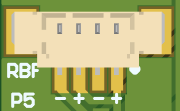
\includegraphics[width=0.25\textwidth]{figures/rbf-picoblades-3d.png}
        \caption{RBF PicoBlade connector on the PCB.}
        \label{fig:rbf-picoblade}
    \end{center}
\end{figure}

\subsection{RTDs PicoBlade} \label{rtd-picoblade}

EPS reads temperature from RTDs present in the BAT4C module with a external PicoBlade cable conected betweem both boards. The two connectors RTD1 and RTD2 pinouts are showed in \autoref{tab:rbf-picoblade} and positions on the PCB in \autoref{fig:rtds-picoblades}.

\begin{table}[!h]
    \centering
    \begin{tabular}{cl}
        \toprule[1.5pt]
        \textit{Pin} & \textit{Row} \\
        \midrule
        RTD1 PicoBlade &  \\
        \midrule
        1            & BAT\_GPIO1   \\
        2            & BAT\_GPIO2   \\
        3            & RTD\_Common  \\
        4            & RTD\_RTD3    \\
        5            & RTD\_Common  \\
        6            & RTD\_RTD2    \\
        7            & RTD\_Common  \\
        8            & RTD\_RTD6    \\
        \midrule
        RTD2 PicoBlade &  \\
        \midrule
        1            & RTD\_Common  \\
        2            & RTD\_RTD5    \\
        3            & RTD\_Common  \\
        4            & RTD\_RTD4    \\
        5            & RTD\_Common  \\
        6            & RTD\_RTD1    \\
        7            & RTD\_Common  \\
        8            & RTD\_RTD0    \\
        \bottomrule[1.5pt]
    \end{tabular}
    \caption{RBF PicoBlade pinout.}
    \label{tab:rbf-picoblade}
\end{table}

\begin{figure}[!ht]
    \begin{center}
        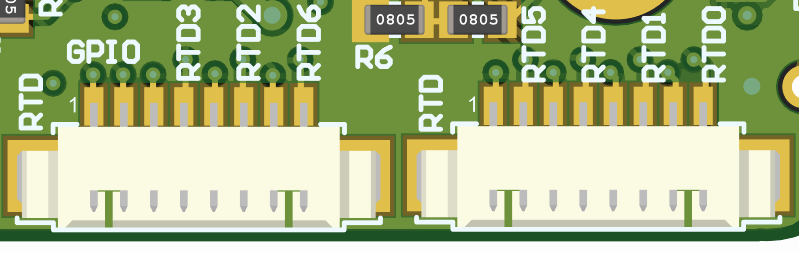
\includegraphics[width=0.45\textwidth]{figures/rtds-picoblades-3d.png}
        \caption{RTDs PicoBlade connectors on the PCB.}
        \label{fig:rtds-picoblades}
    \end{center}
\end{figure}

\subsection{Heater PicoBlade} \label{heater-picoblade}

The PWM signals that control the heaters present on the BAT4C module is also brought by a external PicoBlade cable. The connector pinout is showed in \autoref{tab:heater-picoblade} and positions on the PCB in \autoref{fig:heaters-picoblade}.

\begin{table}[!h]
    \centering
    \begin{tabular}{cl}
        \toprule[1.5pt]
        \textit{Pin} & \textit{Row} \\
        \midrule
        1            & $-$Heater1\_Voltage \\
        2            & $-$Heater1\_Voltage \\
        3            & VBUS \\
        4            & VBUS \\
        5            & $-$Heater2\_Voltage \\
        6            & $-$Heater2\_Voltage \\
        7            & VBUS \\
        8            & VBUS \\
        \bottomrule[1.5pt]
    \end{tabular}
    \caption{Heater PicoBlade pinout.}
    \label{tab:heater-picoblade}
\end{table}

\begin{figure}[!ht]
    \begin{center}
        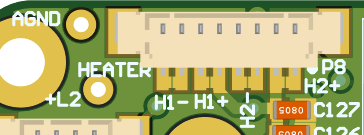
\includegraphics[width=0.4\textwidth]{figures/heaters-picoblade-3d.png}
        \caption{Heaters PicoBlade connector on the PCB.}
        \label{fig:heaters-picoblade}
    \end{center}
\end{figure}

\subsection{External Batteries Charger PicoBlade} \label{external-charge-picoblade}

When the EPS and BAT4C are assembled together the batteries can be charged from a PicoBlade connector on which is acessed in a external interface. The same current restriction as for the solar panels connectors is apllied here, the external batteries charger PicoBlade must not exceed 2000mA. The connector pinout is showed in \autoref{tab:batteries-picoblade} and position on the PCB in \autoref{fig:batteries-picoblade}.

\begin{table}[!h]
    \centering
    \begin{tabular}{cl}
        \toprule[1.5pt]
        \textit{Pin} & \textit{Row} \\
        \midrule
        1            & V\_Charging\_Batteries \\
        2            & V\_Charging\_Batteries \\
        3            & PGND \\
        4            & PGND \\
        \bottomrule[1.5pt]
    \end{tabular}
    \caption{External batteries charger PicoBlade pinout.}
    \label{tab:batteries-picoblade}
\end{table}

\begin{figure}[!ht]
    \begin{center}
        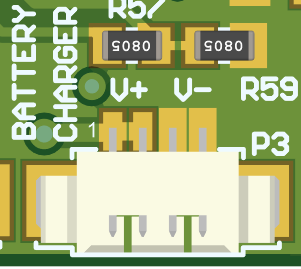
\includegraphics[width=0.25\textwidth]{figures/battery-charger-picoblade-3d.png}
        \caption{External batteries charger PicoBlade connector on the PCB.}
        \label{fig:batteries-picoblade}
    \end{center}
\end{figure}

\subsection{JTAG PicoBlade} \label{jtag-picoblade}

The EPS module can be programed and debugged through its JTAG PicoBlade connector, see \autoref{ch:instructions} for more information regarding right use of this interface. The connector pinout is showed in \autoref{tab:jtag-picoblade} and position on the PCB in \autoref{fig:jtag-picoblade}.

\begin{table}[!h]
    \centering
    \begin{tabular}{cl}
        \toprule[1.5pt]
        \textit{Pin} & \textit{Row} \\
        \midrule
        1            & 3V3\_MCU \\
        2            & TDO \\
        3            & TCK \\
        4            & UART\_Debug\_Tx \\
        5            & UART\_Debug\_Rx \\
        6            & DGND \\
        \bottomrule[1.5pt]
    \end{tabular}
    \caption{JTAG PicoBlade pinout.}
    \label{tab:jtag-picoblade}
\end{table}

\begin{figure}[!ht]
    \begin{center}
        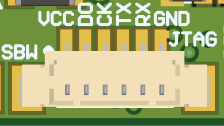
\includegraphics[width=0.35\textwidth]{figures/jtag-picoblade-3d.png}
        \caption{JTAG PicoBlade connector on the PCB.}
        \label{fig:jtag-picoblade}
    \end{center}
\end{figure}

\subsection{Debug UART Pin Header} \label{uart-pin-header}

For debugging via UART using log messages during test phase a pin header can be easily acessed with jumper wires. This connector is not meant to be soldered in the flight model of the EPS. The connector pinout is showed in \autoref{tab:uart-pin-header} and position on the PCB in \autoref{fig:uart-pin-header}.

\begin{table}[!h]
    \centering
    \begin{tabular}{cl}
        \toprule[1.5pt]
        \textit{Pin} & \textit{Row} \\
        \midrule
        1            & UART\_Debug\_Tx \\
        2            & UART\_Debug\_Rx \\
        3            &  DGND \\
        \bottomrule[1.5pt]
    \end{tabular}
    \caption{Debug UART pin header pinout.}
    \label{tab:uart-pin-header}
\end{table}

\begin{figure}[!ht]
    \begin{center}
        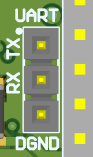
\includegraphics[width=0.15\textwidth]{figures/uart-pin-header-3d.png}
        \caption{Debug UART pin header connector on the PCB.}
        \label{fig:uart-pin-header}
    \end{center}
\end{figure}